\section{Validation}
In order to test our framework, we have assembled a dataset of different types of 3D models, ranging over various applications and various types of geometry.
The dataset is described in detail in the accompanying data in Appendix~\ref{dataset}.
We sliced all models in the dataset and selected 300 random slices from the total set of slices for analysis.
We generated the toolpaths on these 300 outline shapes using the naive technique as implemented by Clipper and compare it to the 4 strategies discussed in \cref{sec_generalization}, namely 'Constant bead count' strategy with a bead count of $C=4$, the 'Centered' beading strategy, the 'Evenly distributed', and the 'Inward distributed' beading strategy, using a nominal bead widths of $w_\text{pref}] = \SI{0.4}{\milli\meter}$.



\subsection{Computational analysis}
Experiments were performed on an Intel Core i7-7500U CPU @ \SI{2.70}{\giga\hertz} using a single core and \SI{16.3}{\giga\byte} memory.
The naive method was implemented using the state-of-the-art polygon offset library Clipper. \cite{johnson2014clipper}
The computation time of each slice from the dataset was recorded for the "Inward distributed" and "Naive" strategy. 
\cref{computime} shows these computation times of each layer plotted against the vertex count of the layer.

The algorithmic complexity is limited by the generation of the Voronoi Diagram, which is $O(n \log n)$, where $n$ is the number of vertices in the input shape.
The number of elements in the ST is linear in the number of elements in the VD
and all of the stages of our framework are also linear in the number of elements in the ST,
so the total running time of our algorithm is $O(n \log n)$.

From the experimental results shown in \cref{computime} we can see that both our framework and the naive method as implemented using Clipper have an expected running time of approximately $2*10^{-5} n \log n$ seconds.
The computation time is approximately five times the computation time of the naive method, which puts it in the same order of magnitude.

% only Moessen reports on computation times, but in a weird manner




\subsubsection{Accuracy}
In order to estimate the overfill and underfill, we need to accurately calculate the area covered by a single extrusion path.
If we would simply use an isosceles trapezoidal area with base lengths equal to the widths of the two end points of the extrusion segment, we would get artifacts at corners in the toolpath (\cref{segment_visualization}a).
We therefore use a semi-circle (\cref{segment_visualization}b) with a diameter equal to the starting width in the one end of each segment, and exclude it at the other end, because it will be included in the next segment.
For polyline extrusion paths which are not closed, we also include the semi-circle corresponding to the extrusion width of the end-position ( \cref{segment_visualization}c).

%In order to print such extrusion paths accurately, we can modulate the amount of material flow per millimeter based on this visualization model.
%See \cref{segment_visualization}.

\begin{figure}
\centering
\setlength{\figwidth}{.25\columnwidth}
\begin{subfigure}{\figwidth}\centering
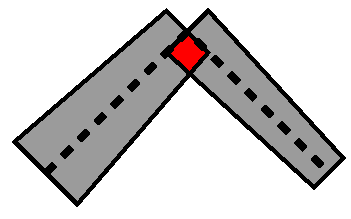
\includegraphics[width=\columnwidth]{sources/validation/visualization_principle_blocky.pdf}
\caption{Blocky}
\end{subfigure}
\begin{subfigure}{\figwidth}\centering
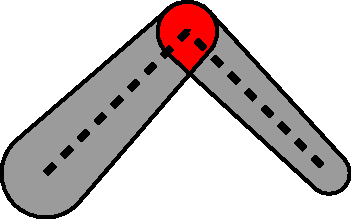
\includegraphics[width=\columnwidth]{sources/validation/visualization_principle_rounded.pdf}
\caption{Rounded}
\end{subfigure}
\begin{subfigure}{\figwidth}\centering
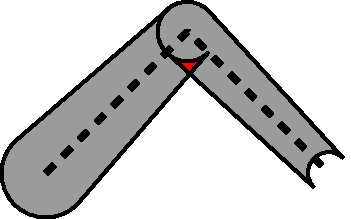
\includegraphics[width=\columnwidth]{sources/validation/visualization_principle_rounded_excluded.pdf}
\caption{Excluded}
\end{subfigure}
\caption{
Extruded area of two extrusion extrusion segments.
Red areas signify doubly extruded areas.
}
\label{segment_visualization}
\end{figure}

We can then estimate the amount of underfill by unioning the rounded visualization of all extrusion segments and then taking the difference from the original outline shape.
In order to deal with rounding errors, we perform a morphological close of \SI{5}{\micro\meter} before calculating the total area of the underfill regions.

The overfill regions are calculated by adding the polygonal areas of each extrusion segment to a list.
We then add the original outline shape in reverse and perform a Vatti clipping operation \cite{Vatti2019clipping} which only keeps areas of positive winding number.
Because the reverse outline shape reduces the winding number of all extruded segments by one, only the overfill areas are left with a positive winding number.
In order to estimate the areas which are triply covered by extrusion segments, we repeat the process of adding the outline in reverse and performing Vatti's clipping operation.
These triple extrusion areas count double toward the total amount of overfill.
The resulting overfill and underfill areas are visualized for the different toolpath strategies in the top of \cref{visualized_accuracy}.


\begin{figure*}
\centering
\setlength{\figwidth}{0.19\textwidth}
\setlength{\figheight}{0.283\textwidth}
\begin{subfigure}{\figwidth}\centering
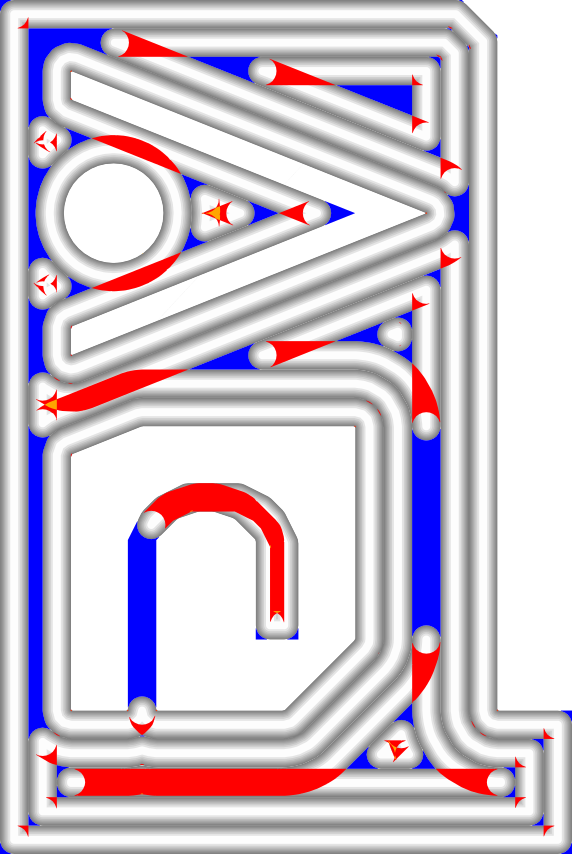
\includegraphics[height=\figheight]{sources/validation/gMAT_example/TEST_naive_accuracy.png}
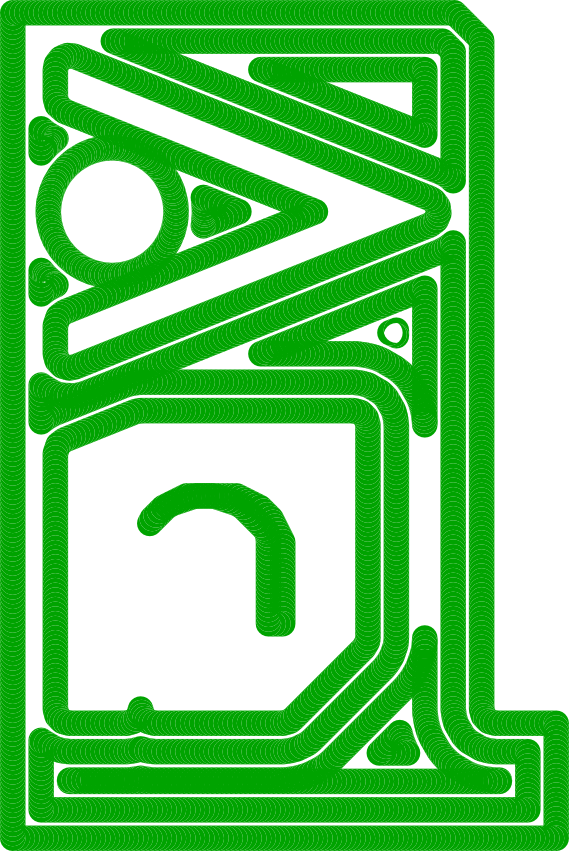
\includegraphics[height=\figheight]{sources/validation/gMAT_example/TEST_naive_widths.png}
\caption{Naive}\label{TEST_naive_accuracy}
\end{subfigure}
%\begin{subfigure}{\figwidth}\centering
%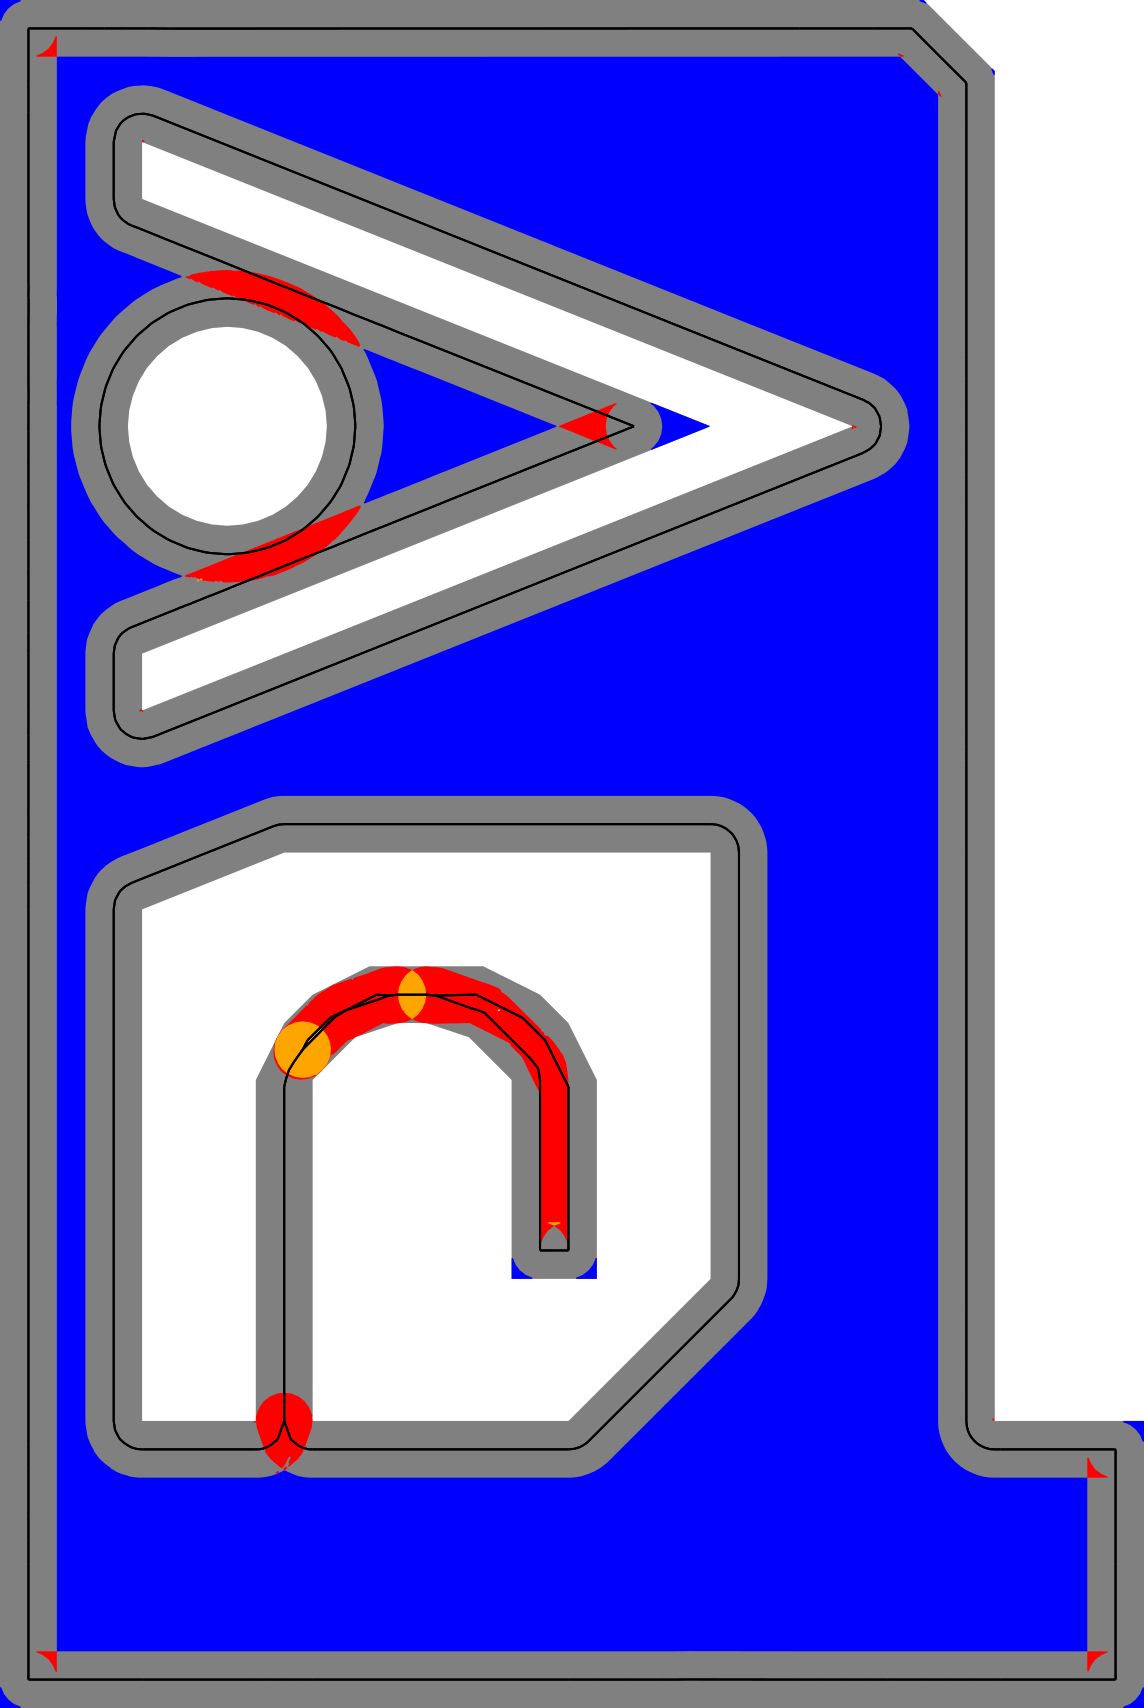
\includegraphics[height=\figheight]{sources/validation/gMAT_example/TEST_SingleBead_accuracy.png}
%
\includegraphics[height=\figheight]{sources/validation/gMAT_example/TEST_SingleBead_widths.png}
%\caption{Single}\label{TEST_SingleBead_accuracy}
%\end{subfigure}
\begin{subfigure}{\figwidth}\centering
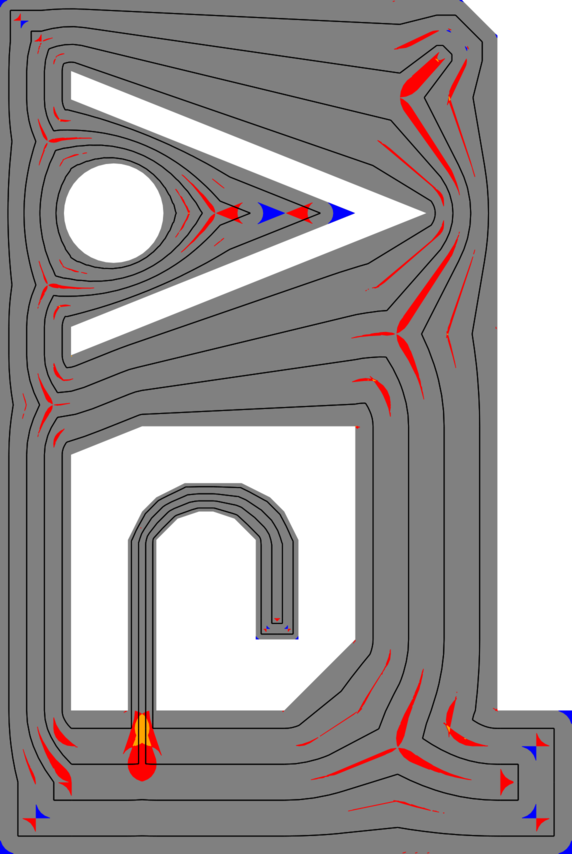
\includegraphics[height=\figheight]{sources/validation/gMAT_example/TEST_Constant_accuracy.png}
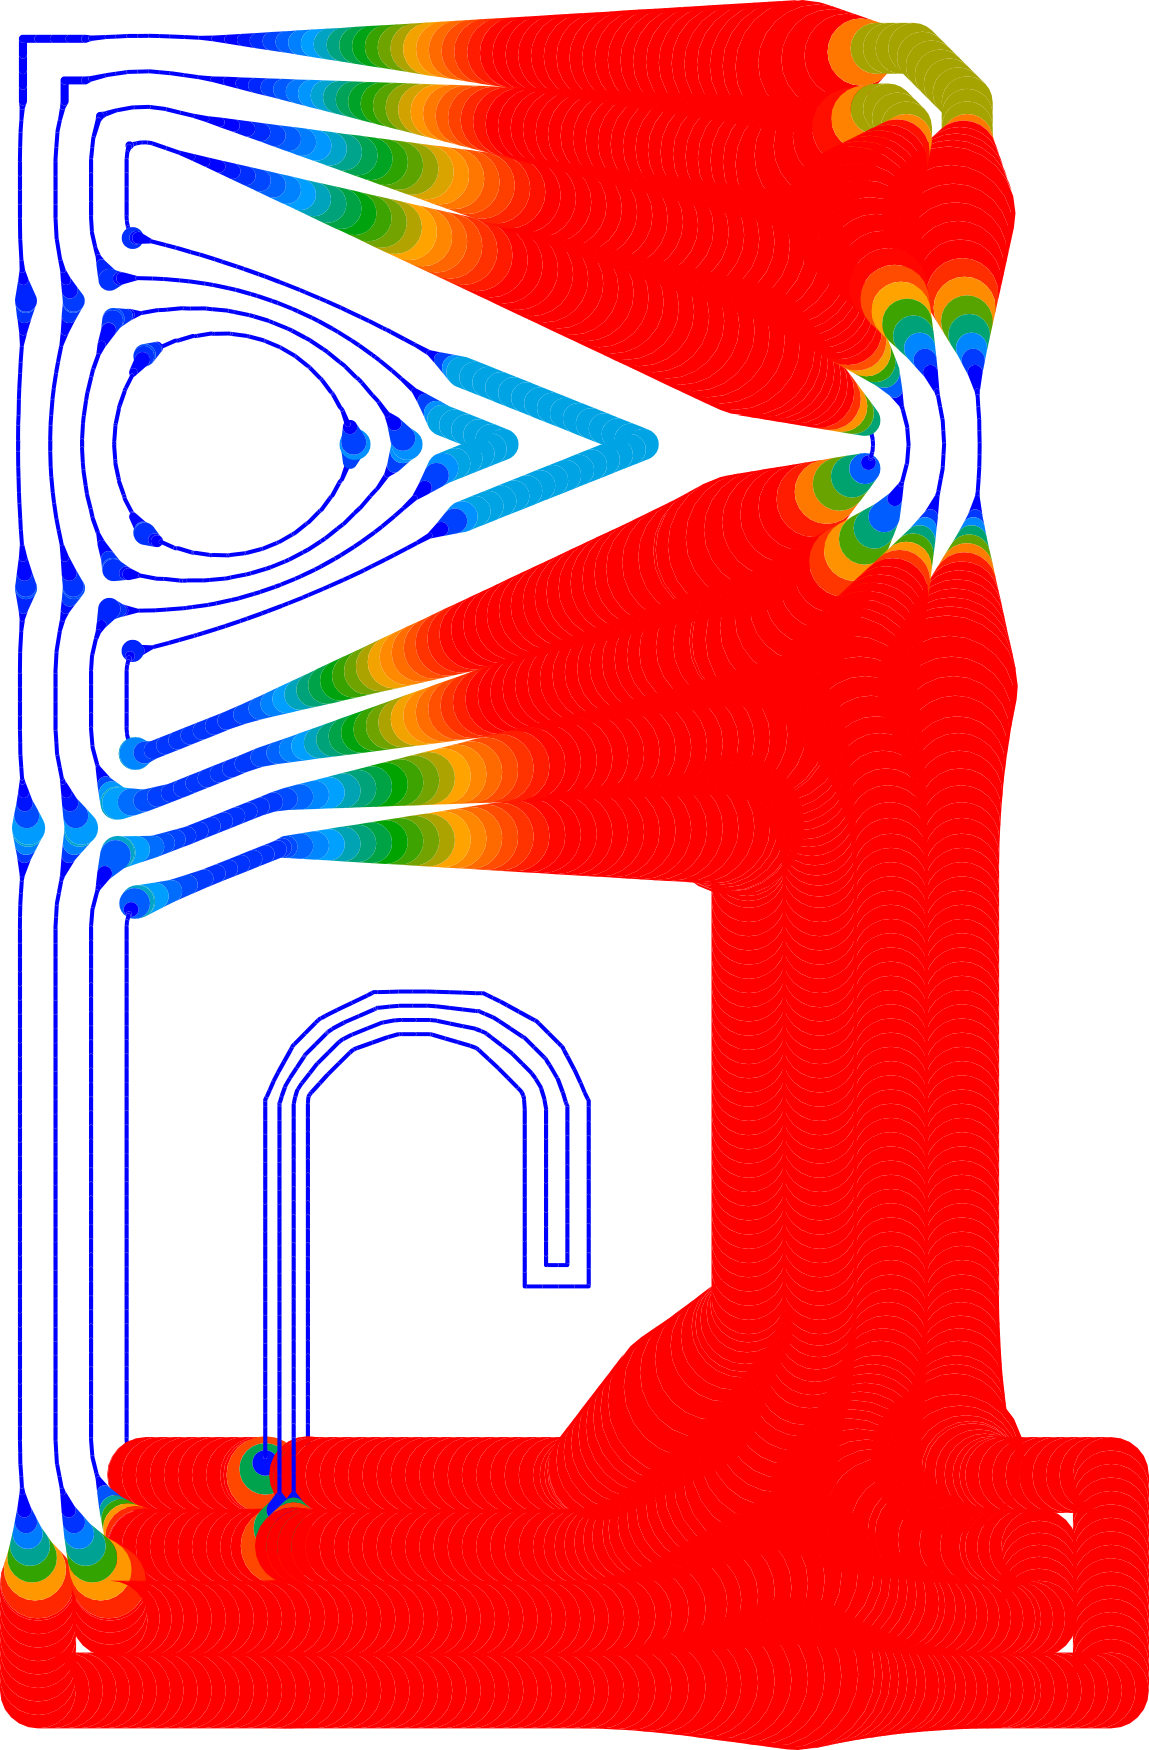
\includegraphics[height=\figheight]{sources/validation/gMAT_example/TEST_Constant_widths.png}
\caption{Constant}\label{TEST_Constant_accuracy}
\end{subfigure}
\begin{subfigure}{\figwidth}\centering
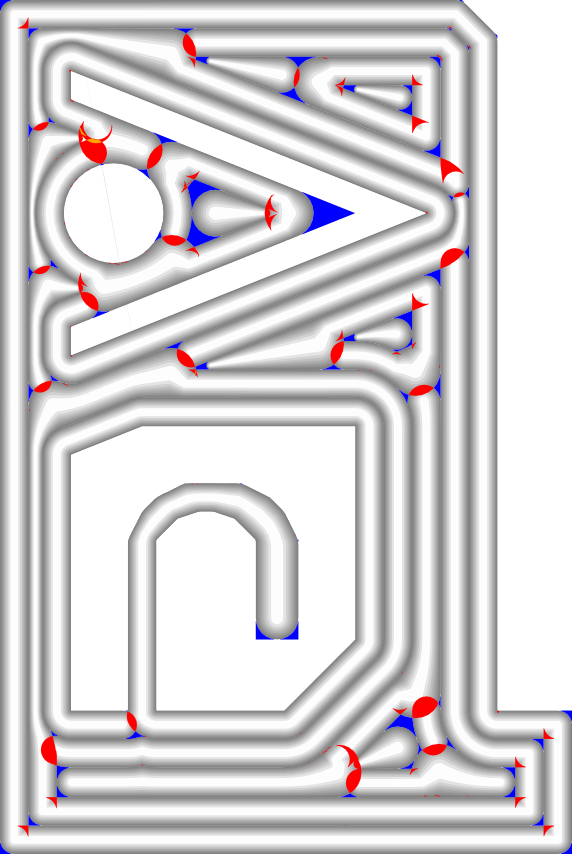
\includegraphics[height=\figheight]{sources/validation/gMAT_example/TEST_Center_accuracy.png}
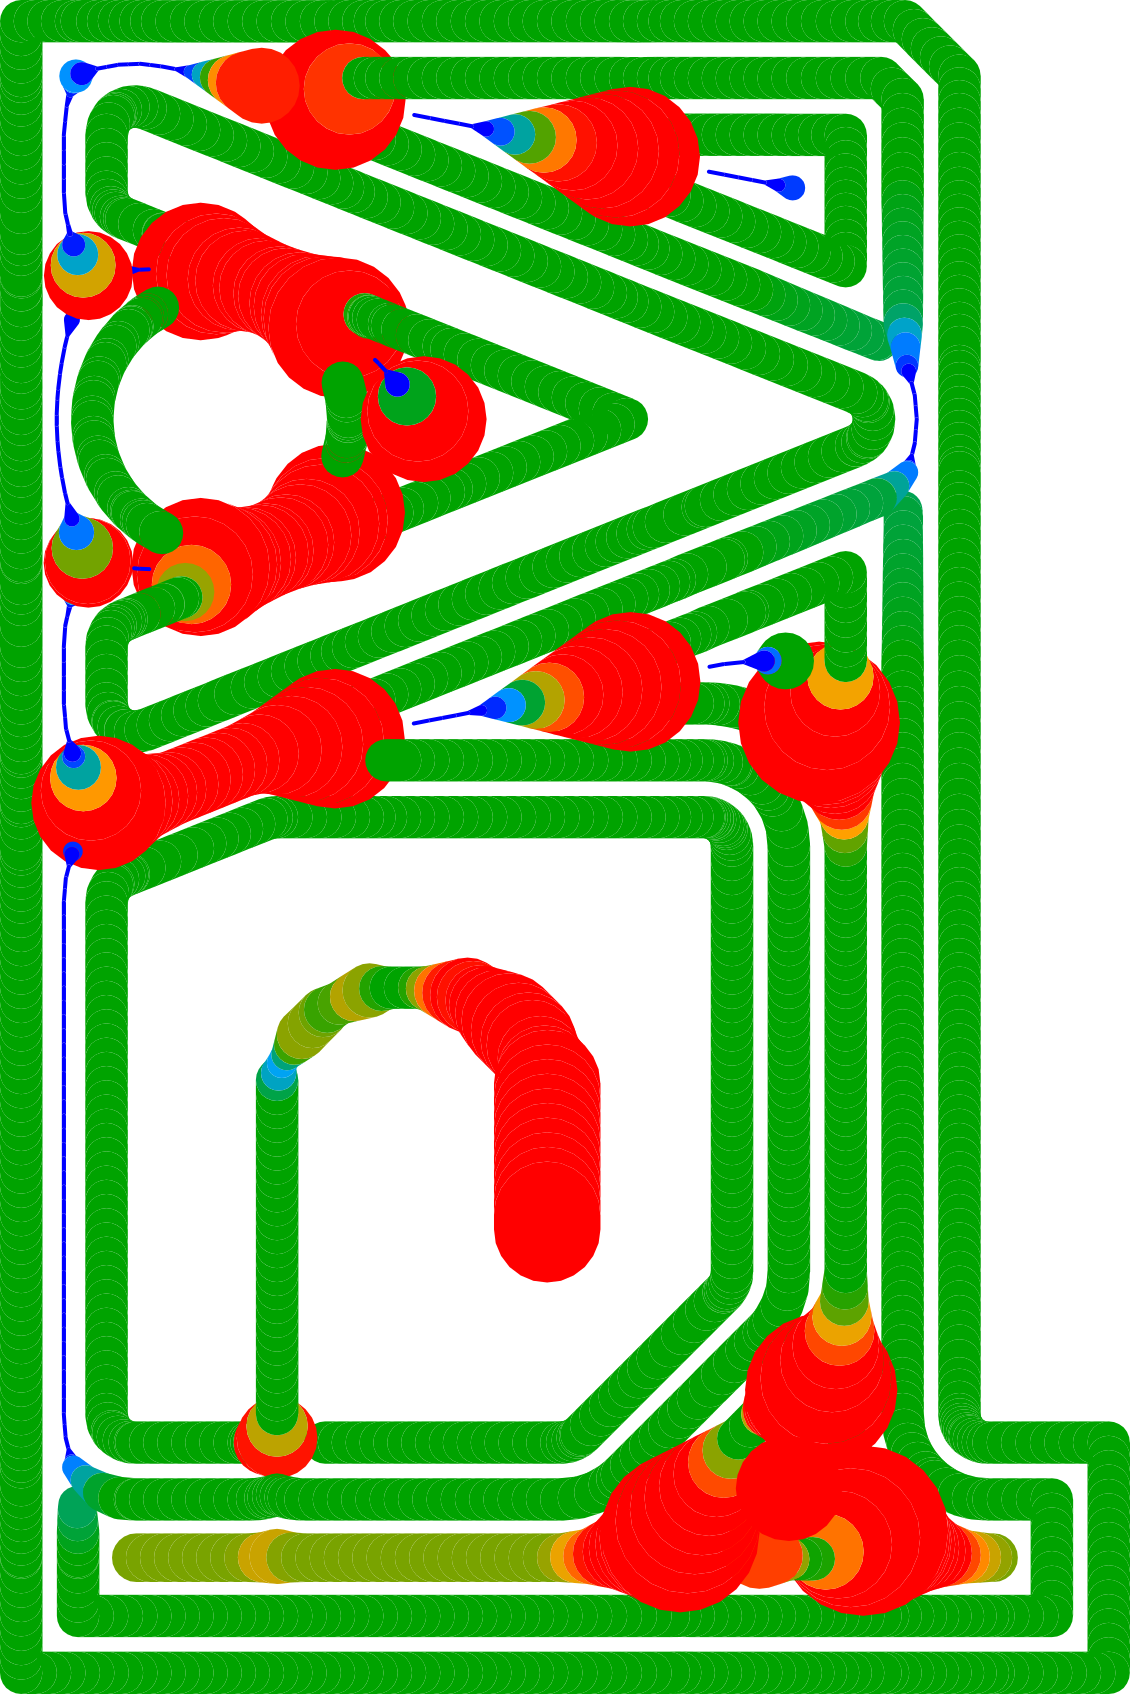
\includegraphics[height=\figheight]{sources/validation/gMAT_example/TEST_Center_widths.png}
\caption{Center}\label{TEST_Center_accuracy}
\end{subfigure}
\begin{subfigure}{\figwidth}\centering
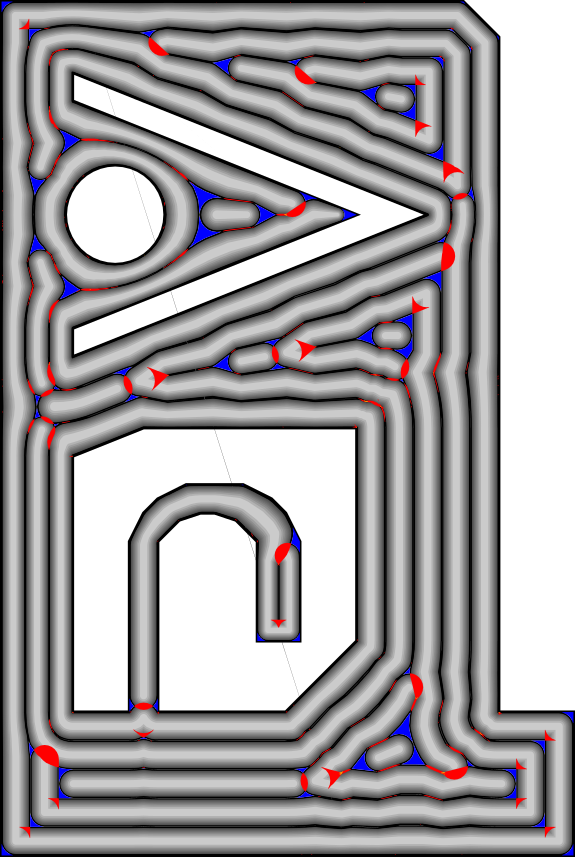
\includegraphics[height=\figheight]{sources/validation/gMAT_example/TEST_Distributed_accuracy.png}
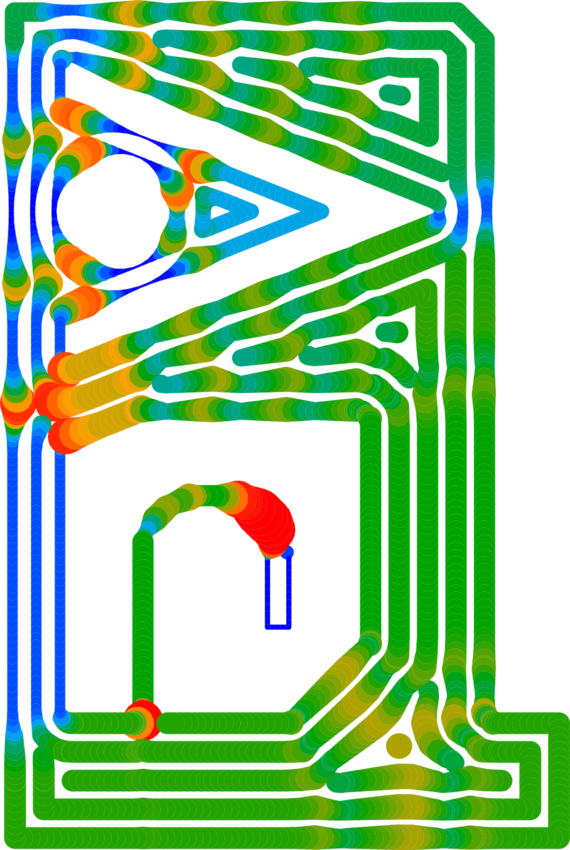
\includegraphics[height=\figheight]{sources/validation/gMAT_example/TEST_Distributed_widths.png}
\caption{Distributed}\label{TEST_Distributed_accuracy}
\end{subfigure}
\begin{subfigure}{\figwidth}\centering
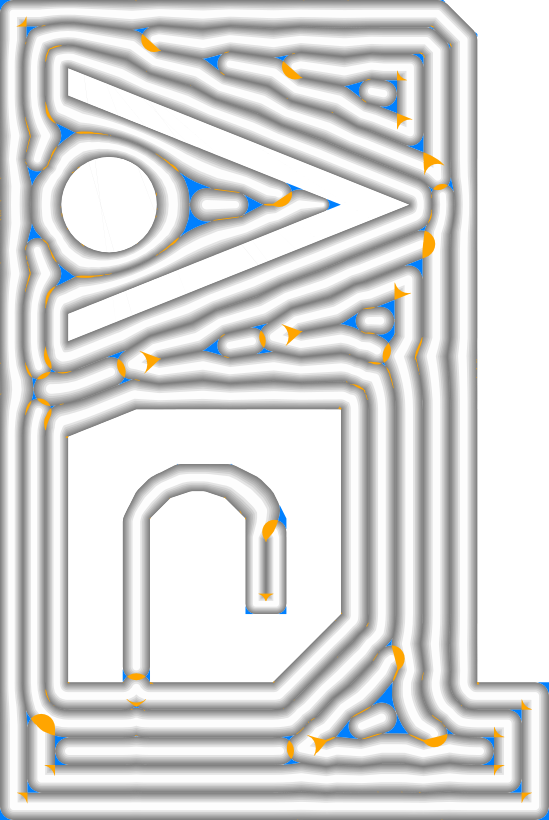
\includegraphics[width=\columnwidth]{sources/validation/gMAT_example/TEST_InwardDistributed_accuracy.png}
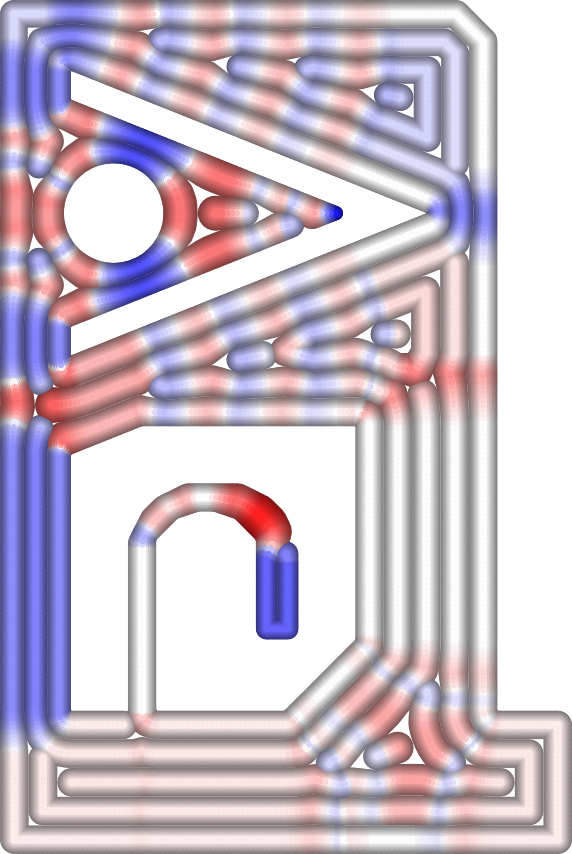
\includegraphics[width=\columnwidth]{sources/validation/gMAT_example/TEST_InwardDistributed_widths.png}
\caption{Inward}\label{TEST_InwardDistributed_accuracy}
\end{subfigure}
\begin{subfigure}{.04\columnwidth}\centering
\vspace{4.7cm}
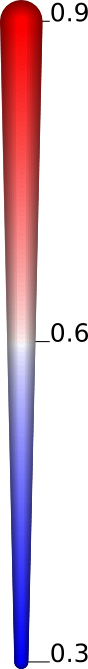
\includegraphics[height=\figheight]{sources/validation/gMAT_example/widths_legend.png}
\end{subfigure}
\caption{
Visualizing the overfills and underfills and the widths for various beading strategies.
Extrusion beads in gray tones,
overfill in orange,
underfill in azure,
narrow beads in blue
and wide beads in red.
}
\label{visualized_accuracy}
\end{figure*}


We calculated the total overfill and underfill areas of the different toolpath strategies applied on the dataset. 
The overfill and underfill areas as a percentage of the total area of the slices from the dataset are illustrated in \cref{over_underfill}.  
The "Inward distributed" strategy has a calculated overfill of 0.24\% and an underfill of 0.17\%.
This is lower compared to the "Naive" strategy, which results in 1.2\% overfill and 1.7\% underfill when applied to the dataset.

\begin{figure*}
\centering
\setlength{\figheight}{0.2\textwidth}
\setlength{\figwidth}{0.31\textwidth}
\begin{subfigure}{\figwidth}\centering
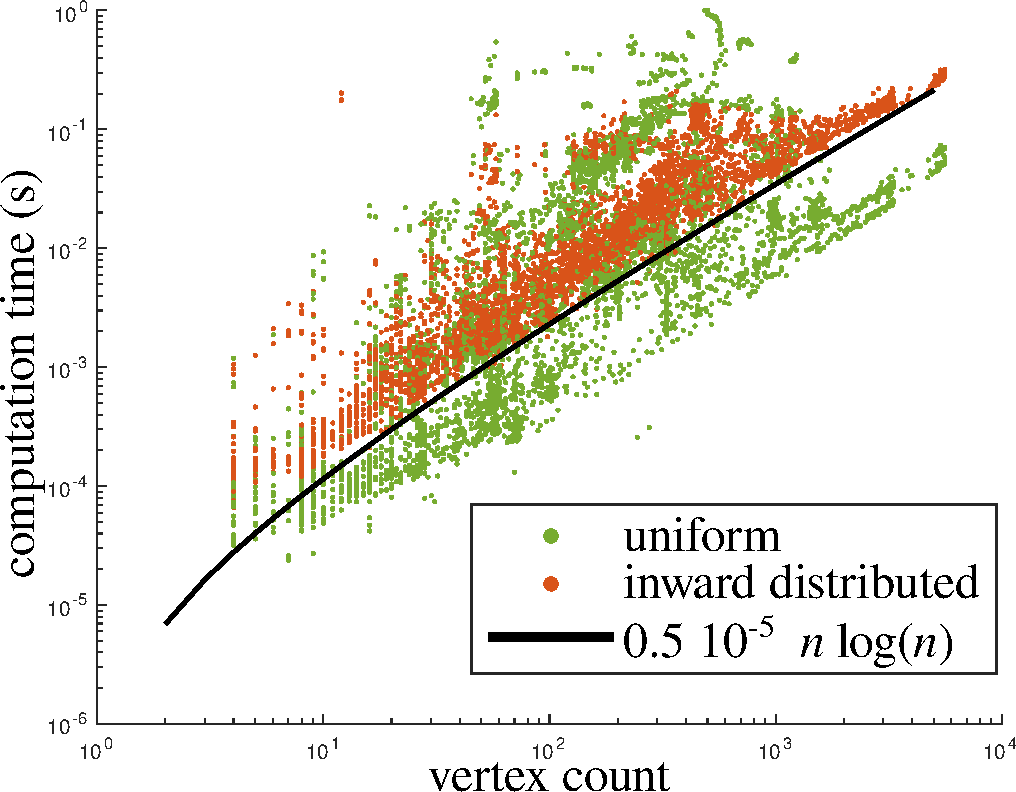
\includegraphics[height=\figheight]{sources/validation/computime2.pdf}
%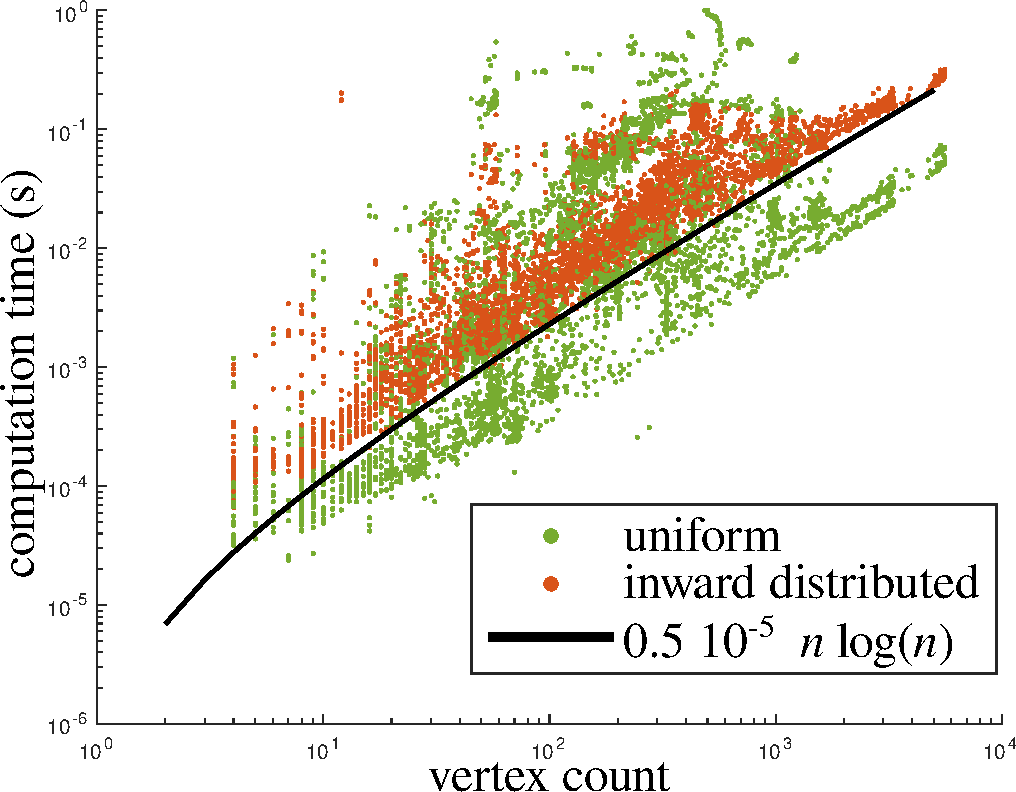
\includegraphics[width=\figwidth]{sources/validation/computime2.pdf}
\caption{Computation time and target vertex count for the full dataset}
\label{computime}
\end{subfigure}
\begin{subfigure}{\figwidth}\centering
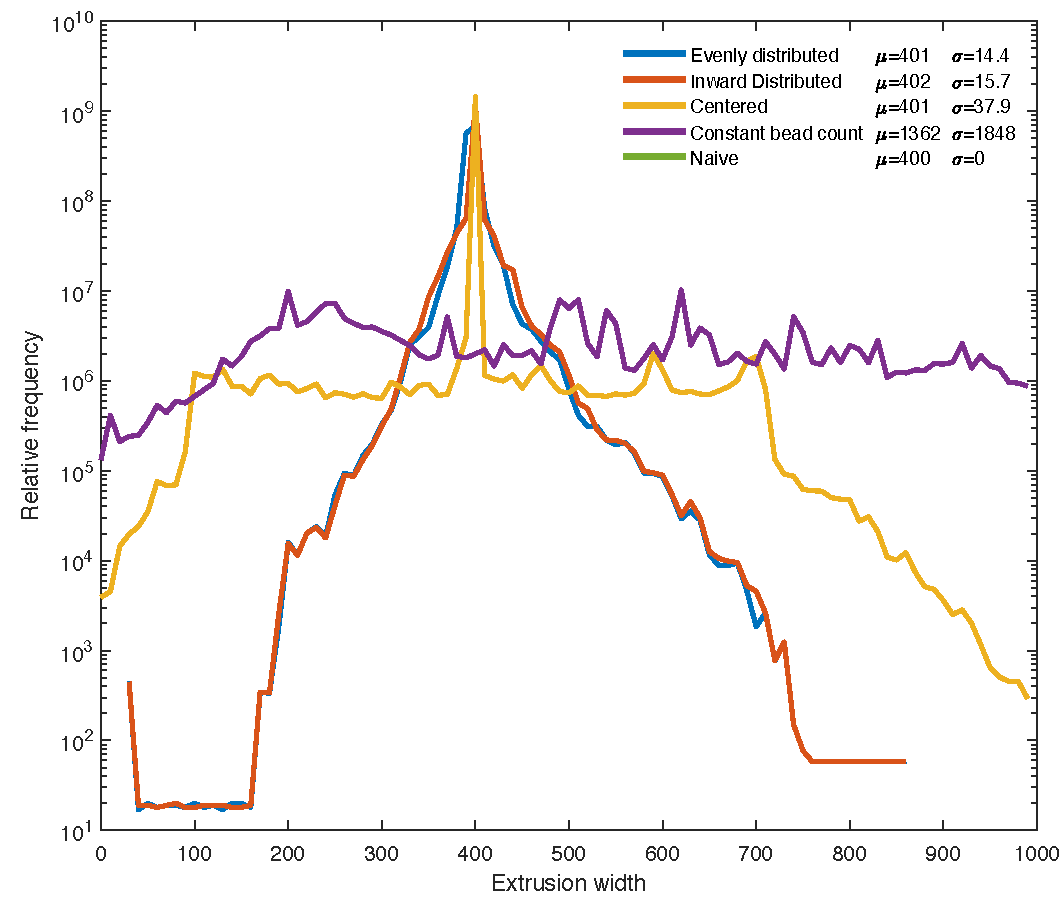
\includegraphics[height=\figheight]{sources/validation/widthHistogram.pdf}
%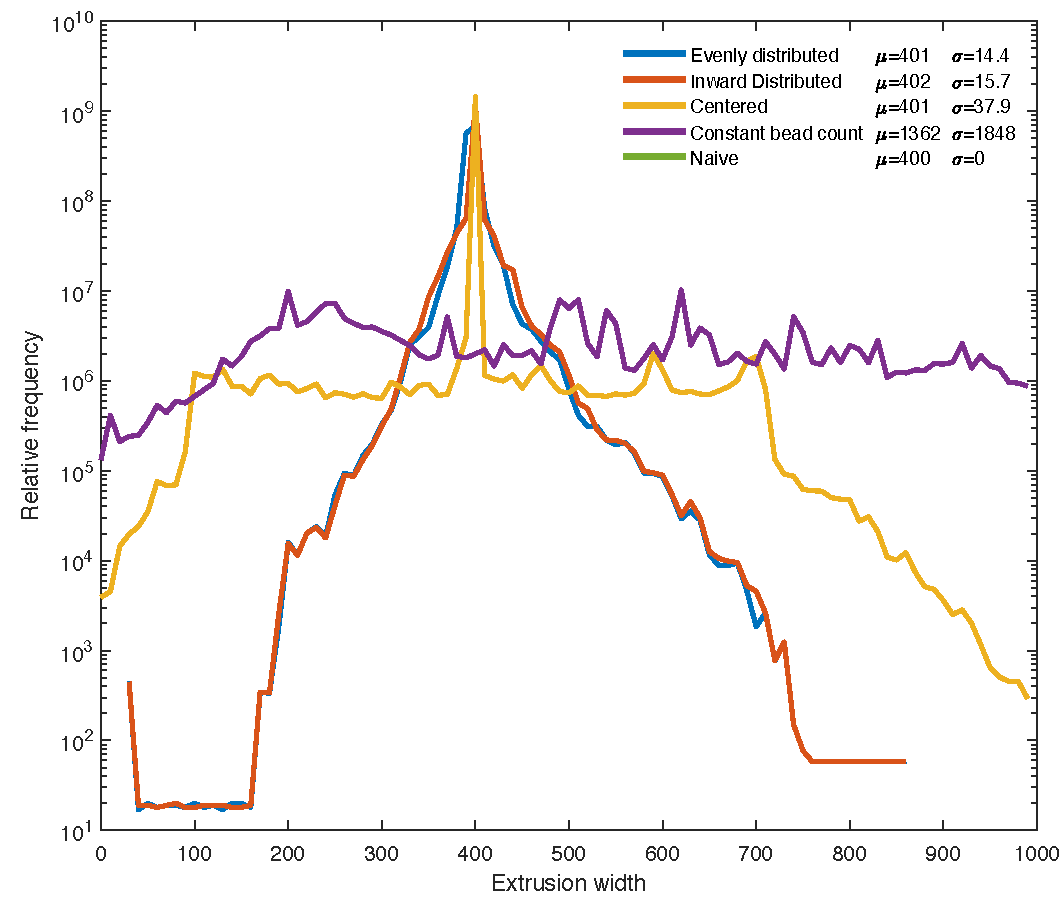
\includegraphics[width=\figwidth]{sources/validation/widthHistogram.pdf}
\caption{Relative frequency of extrusion widths}
\label{widthHistogram}
\end{subfigure}
\begin{subfigure}{\figwidth}\centering
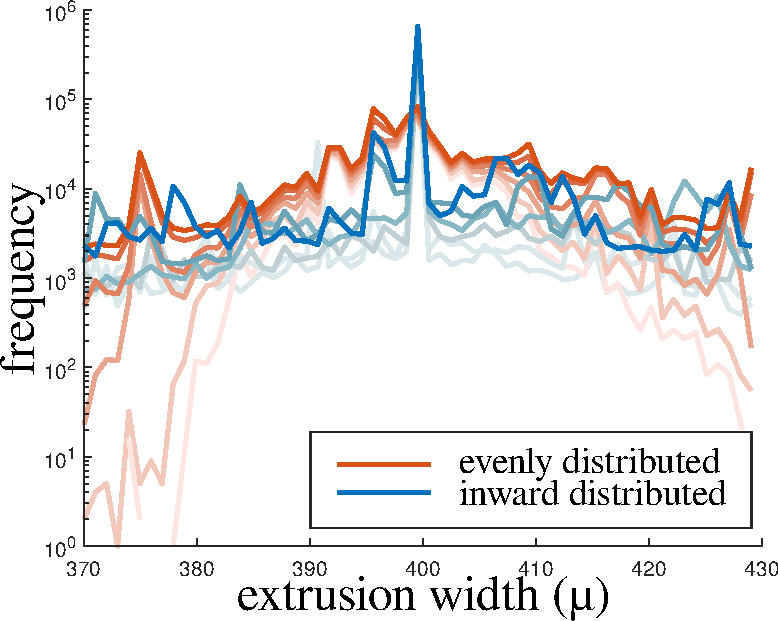
\includegraphics[height=\figheight]{sources/validation/indexedwidths2.pdf}
%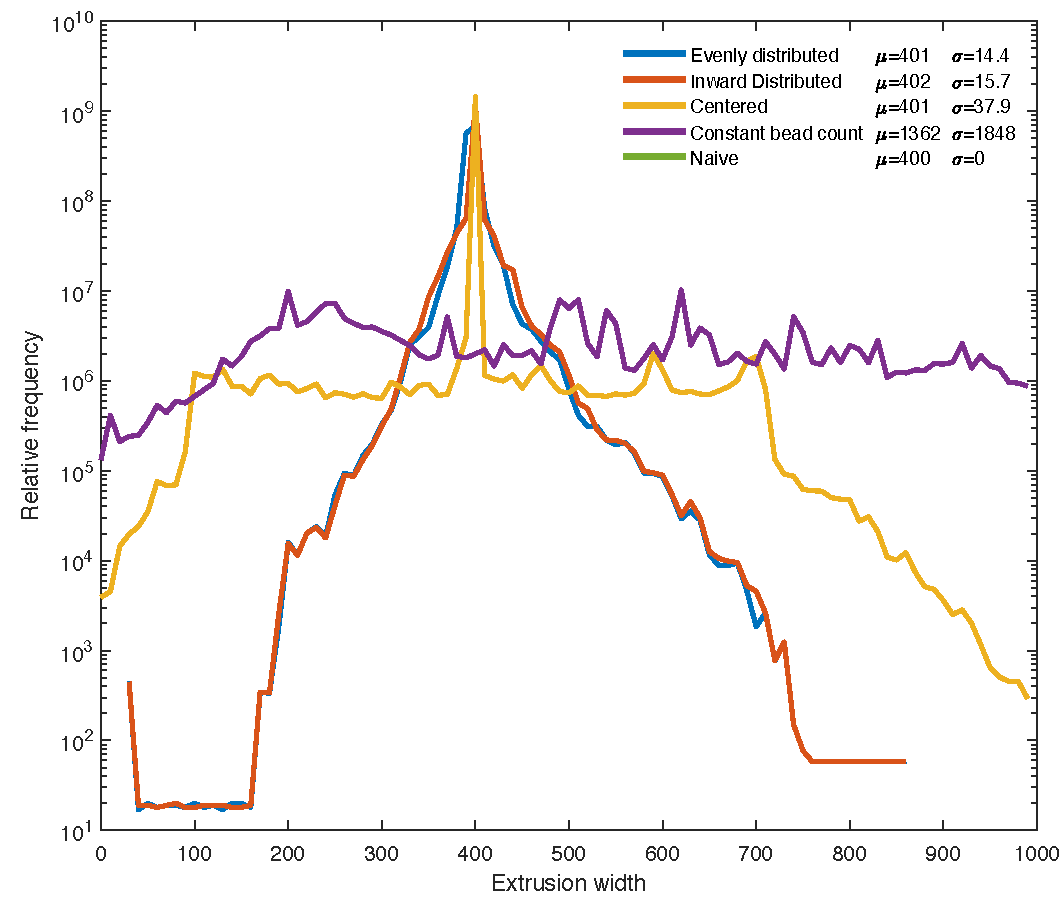
\includegraphics[width=\figwidth]{sources/validation/widthHistogram.pdf}
\caption{Relative frequency of extrusion widths for 6 outer contours}
\label{widthIndexedHistogram}
\end{subfigure}
\begin{subfigure}{\figwidth}\centering
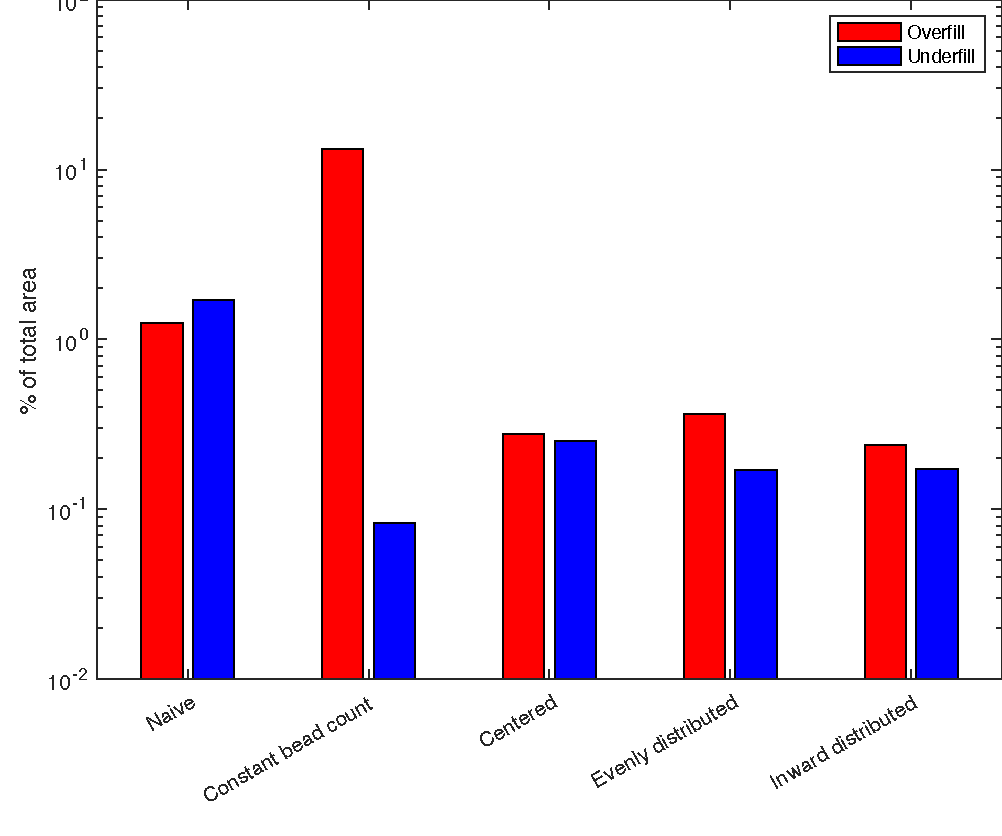
\includegraphics[height=\figheight]{sources/validation/overunderfill.pdf}
%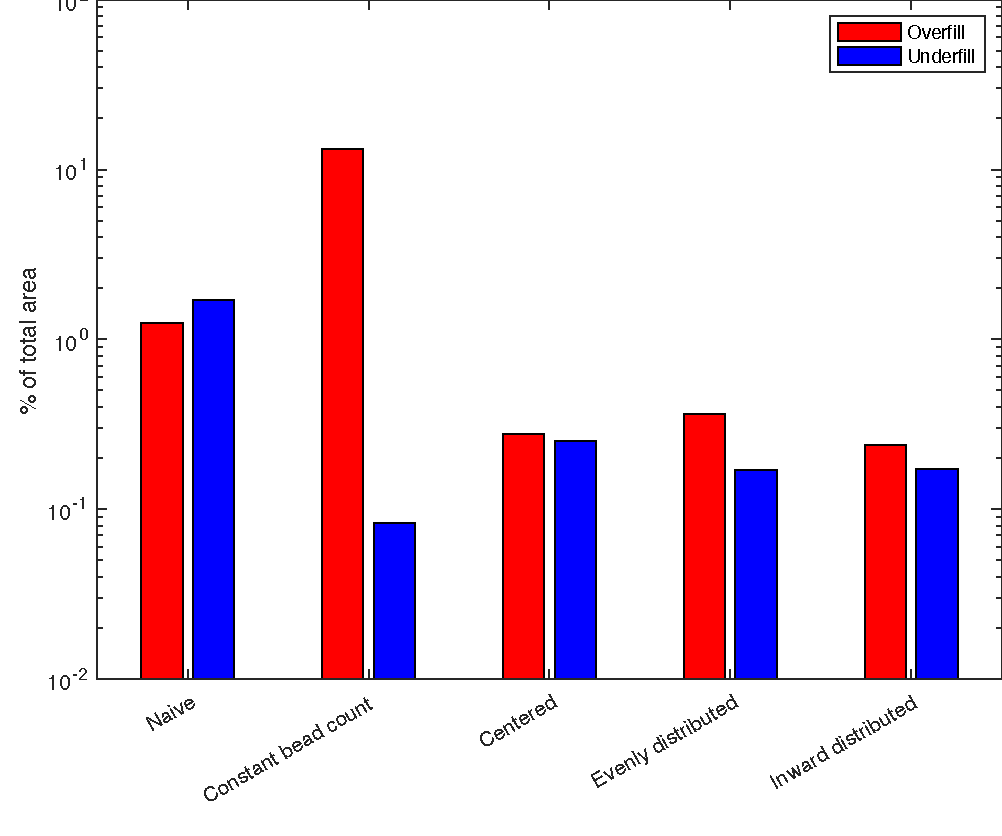
\includegraphics[width=\figwidth]{sources/validation/overunderfill.pdf}
\caption{Total over and underfill area}
\label{over_underfill}
\end{subfigure}
\begin{subfigure}{\figwidth}\centering
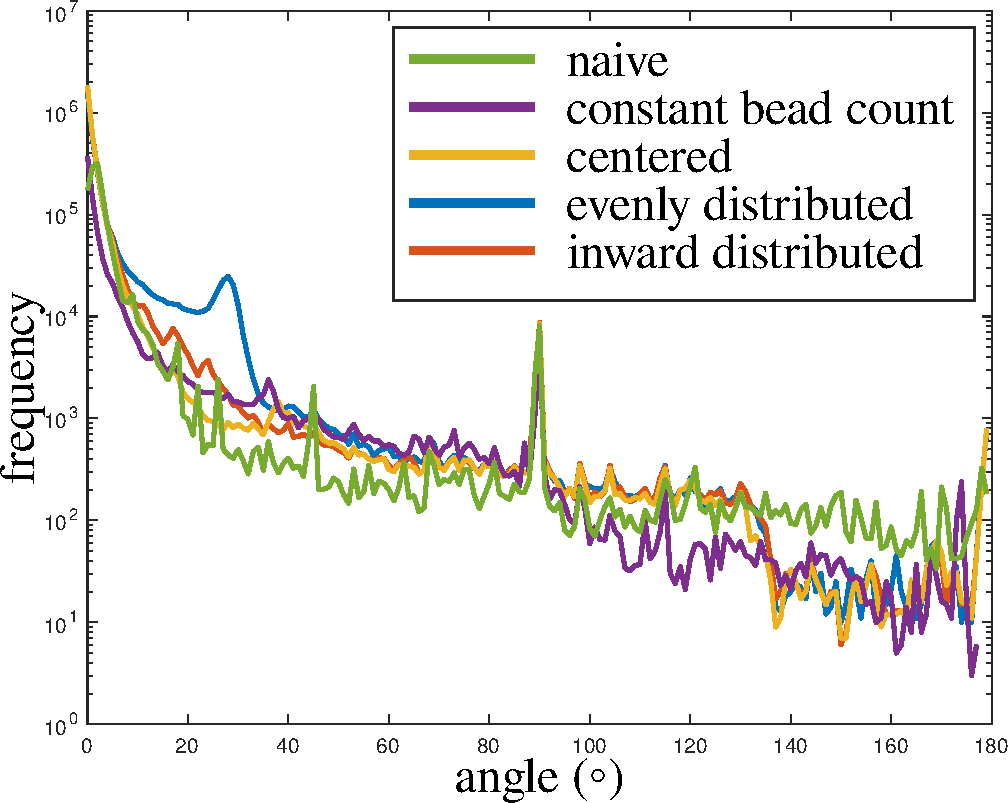
\includegraphics[height=\figheight]{sources/validation/smoothness.pdf}
%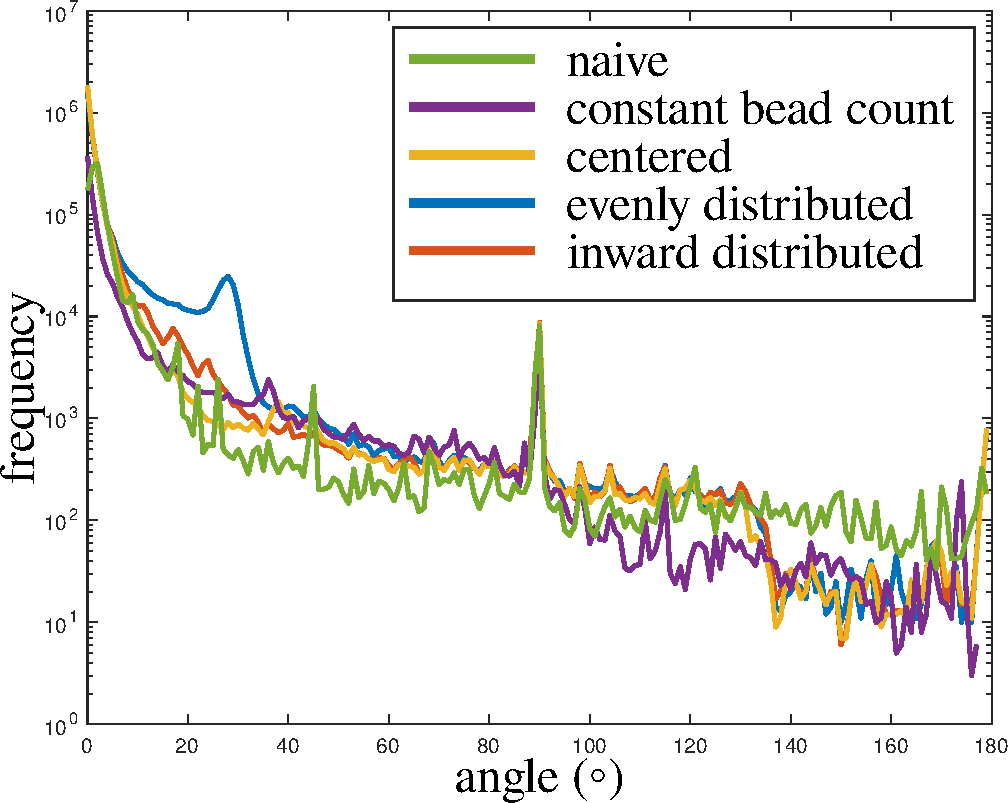
\includegraphics[width=\figwidth]{sources/validation/smoothness.pdf}
\caption{Frequency of angles between consecutive segments}
\label{smoothness}
\end{subfigure}
\begin{subfigure}{\figwidth}\centering
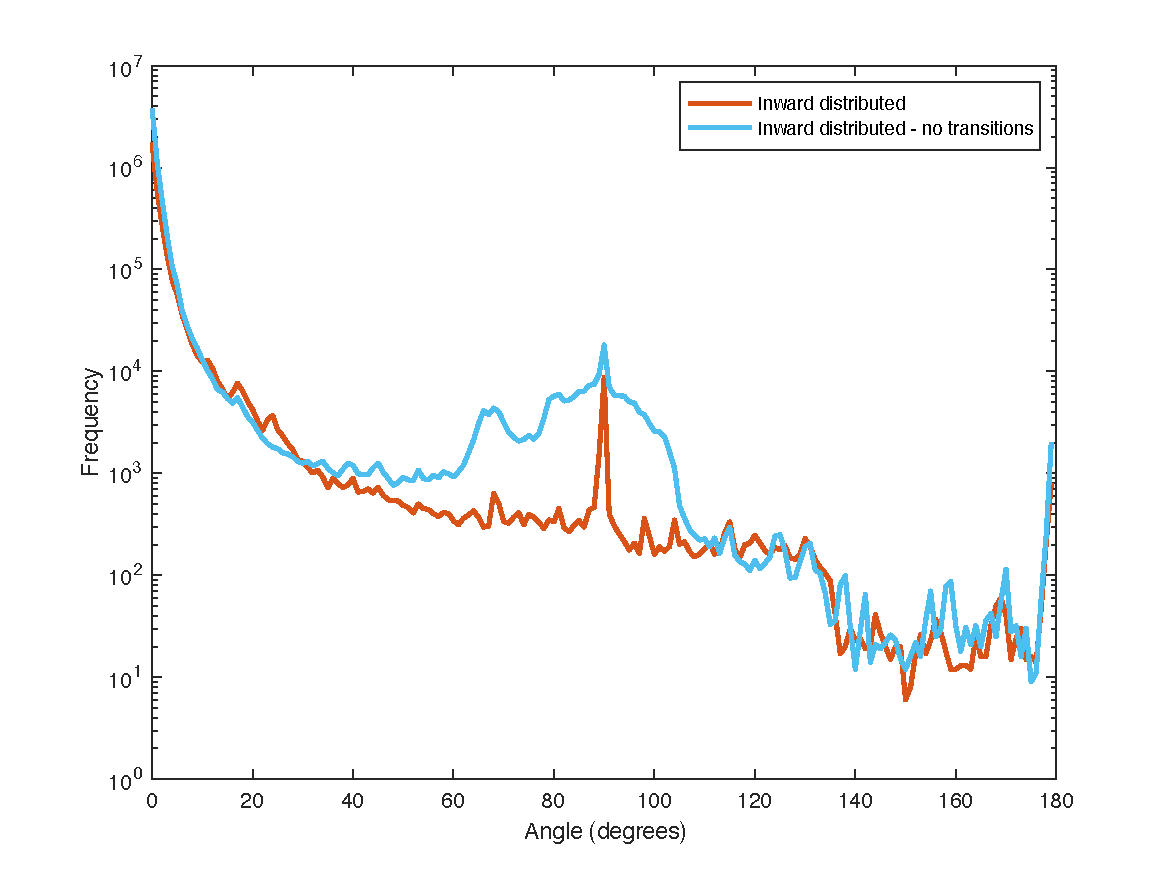
\includegraphics[height=\figheight]{sources/validation/smoothnessNoTransition.pdf}
%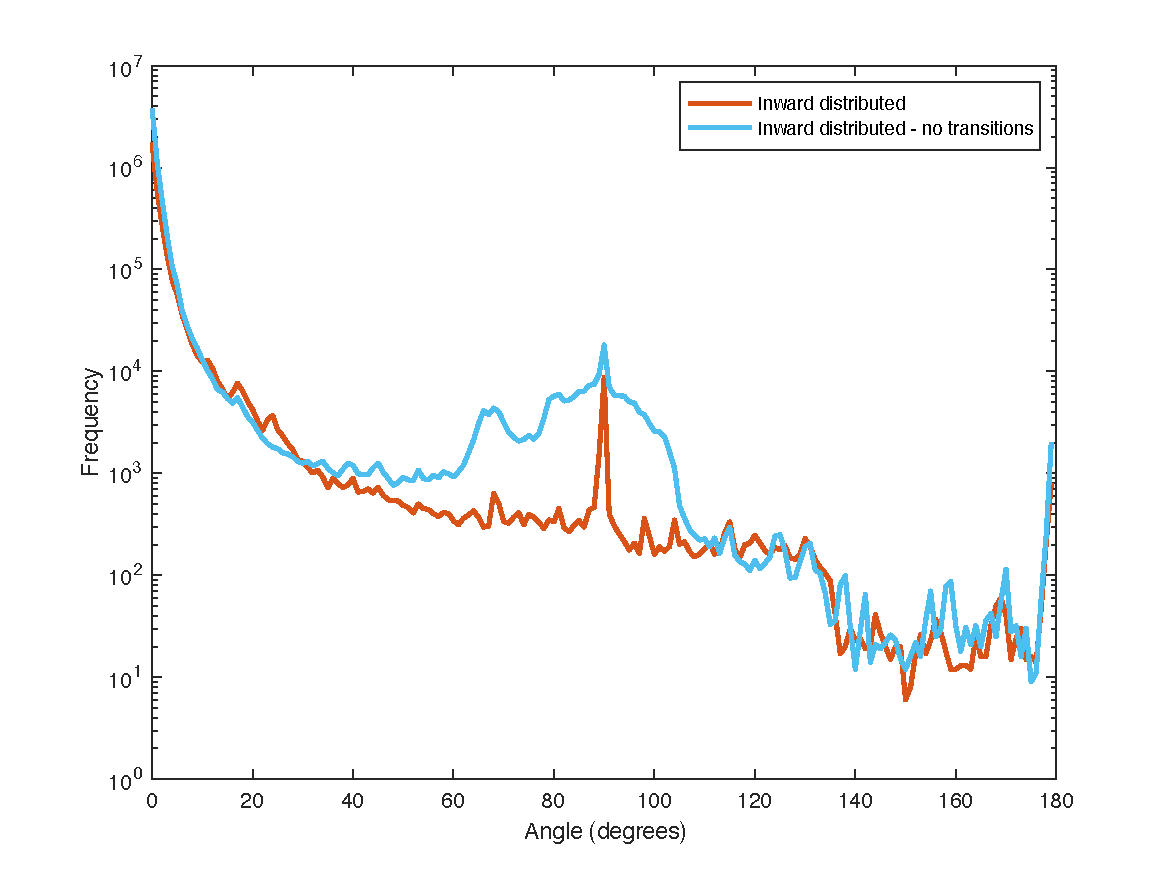
\includegraphics[width=\figwidth]{sources/validation/smoothnessNoTransition.pdf}
\caption{Frequency of angles with and without transitions}
\label{smoothnessNoTransition}
\end{subfigure}


\caption{
Results of computational analysis of the results from applying the naive method and various beading strategies using our framework to the dataset.
Note the use of a logarithmic scale on the Y-axes and on some of the X-axes as well.
}
\end{figure*}









\subsubsection{Uniformity}
Depending on the printer hardware configuration, some bead widths might be difficult or impossible to produce.
A bead width far below the nozzle size can result in fluttered extrusion, while a bead width far above the nozzle size can require pressures above the specifications of the machine. 
Also, large bead widths may cause the extruded material to bulge upwards instead of filling the required width.
Moreover, bead widths deviating from the nominal bead width by a large amount may impact the mechanical properties of the print.
We visualize the bead widths resulting from the different strategies in the bottom of \cref{visualized_accuracy}.

To evaluate the width uniformity, we sampled the extrusion widths of all generated toolpaths 
at intervals of \SI{1}{\micro\meter} along the toolpath.
From these sampled values, we calculated the mean bead width, and standard deviation per strategy.
\cref{widthHistogram} shows the distribution of extrusion width for each strategy binned at intervals of \SI{10}{\micro\meter}.
We found that the mean width of our strategies 'Inward distributed' and 'Evenly distributed' is close to nominal nozzle size of \SI{400}{\micro\meter}, while their standard deviation is lower than for strategies 'Centered' and 'Constant bead count'. 
These results indicate that, while causing less overfill and underfill, 'Inwards distributed' and 'Evenly distributed' strategies deviate less and infrequently from the nominal nozzle size compared to the other strategies.
We compared the width uniformity of the 6 outer beads for the strategies 'Inward distributed' and 'Evenly distributed', the distribution of these extrusion widths is shown in \cref{widthIndexedHistogram}. 
The outer beads of the 'Inward distributed' strategy clearly have more often the nominal width of \SI{400}{\micro\meter}, while the 'Evenly distributed' more often extrudes widths that deviate from the nominal width.

\paragraph{Smoothness of toolpaths}
In order to maintain a high printing speed, it is desirable that toolpaths have fewer and less sharp corners. 
We measured the angle between consecutive extrusion segments generated by each strategy.
The relative frequency of these angles is shown in \cref{smoothness}.
All strategies show a higher number of corners for smaller angles with a peak towards 0 degrees (straight line).
The 'Inward distributed' strategy produces an order of magnitude less corners around 30 degrees, compared to 'Evenly distributed'. 
We also investigated the effect of the transition regions on the smoothness of the toolpaths. 
\cref{smoothnessNoTransition} shows that introducing the transitions greatly reduces the number of corners around 90 degrees. 

\subsection{Experimentation}
Test prints were performed on a custom FDM hardware setup, with a standard \SI{0.4}{\milli\meter} nozzle and a filament extrusion drive directly mounted on the print head.
The firmware of the printer employs linear advance: to gain the extra pressure required to change to a wider bead an extra amount of filament is advanced into the physical system between the filament feeder and the nozzle so that we can realize accurate adaptive deposition width control.\cite{tronvoll2019investigating}
We set the preferred width to $w_\text{pref} = \SI{0.6}{\milli\meter}$, so that we avoid fluttered printing of lines thinner than the nozzle size.
We used a layer thickness of \SI{0.2}{\milli\meter} and a movement speed of \SI{10}{\milli\meter\per\second}.

The resulting prints are shown in \cref{wedge_print} and \cref{prints}.
Because of inaccuracies in the depositioning control system some of the prints show defects.
Such defects are less prevalent for the inward distributed beading strategy than the other strategies.


\begin{figure}
\centering
\begin{subfigure}{\columnwidth}\centering
\setlength{\figwidth}{\columnwidth}
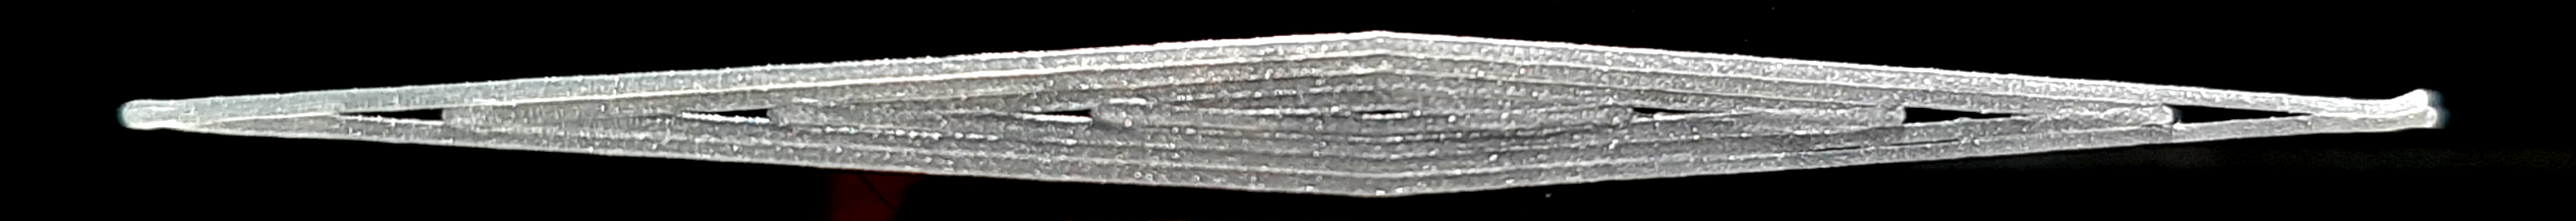
\includegraphics[width=\figwidth]{sources/applications/P3_print_wedge_naive_edited.png}
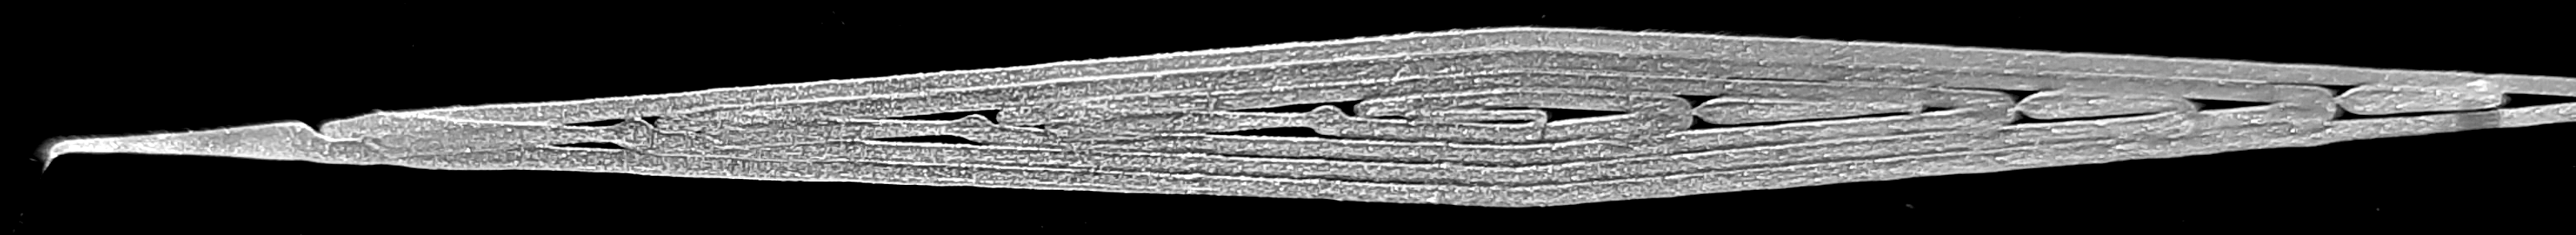
\includegraphics[width=\figwidth]{sources/applications/P3_print_wedge_center_edited.png}
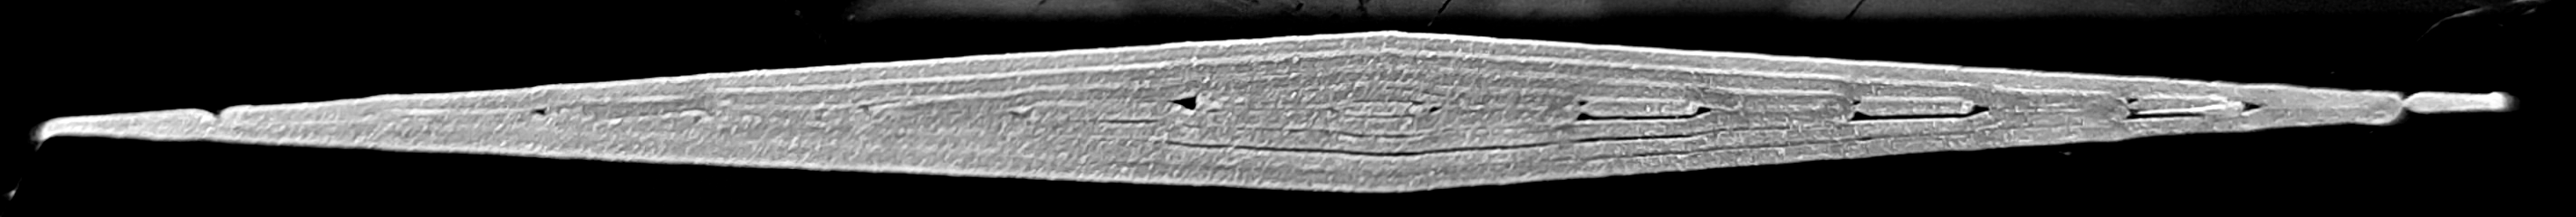
\includegraphics[width=\figwidth]{sources/applications/P3_print_wedge_inward_edited.png}
\caption{Wedge}\label{print_wedge}
\end{subfigure}
\caption{
A wedge shape printed using the naive strategy, center deivation strategy and the inward distributed strategy.
The naive and center deviation strategy show problems around certain model diameters.
}
\label{wedge_print}
\end{figure}

\begin{figure}
\centering
\setlength{\figheight}{.38\columnwidth}
\setlength{\figheightTwo}{.47\columnwidth}
\setlength{\figwidth}{0.32\columnwidth}
\begin{subfigure}{\figwidth}\centering
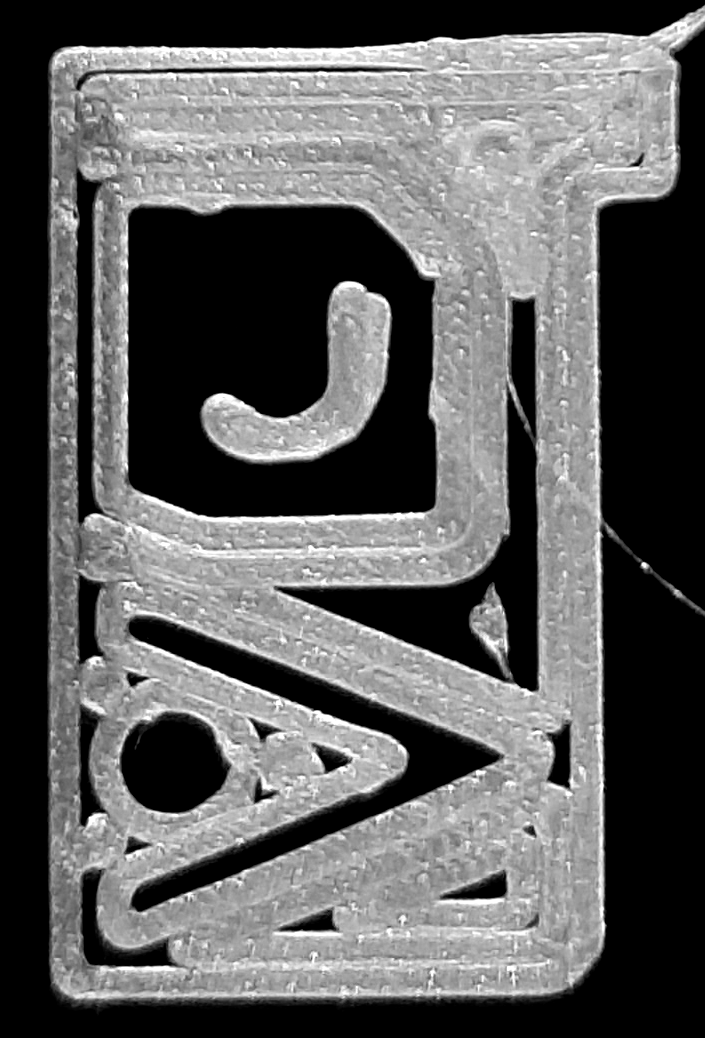
\includegraphics[height=\figheightTwo]{sources/applications/gMAT_naive.png}
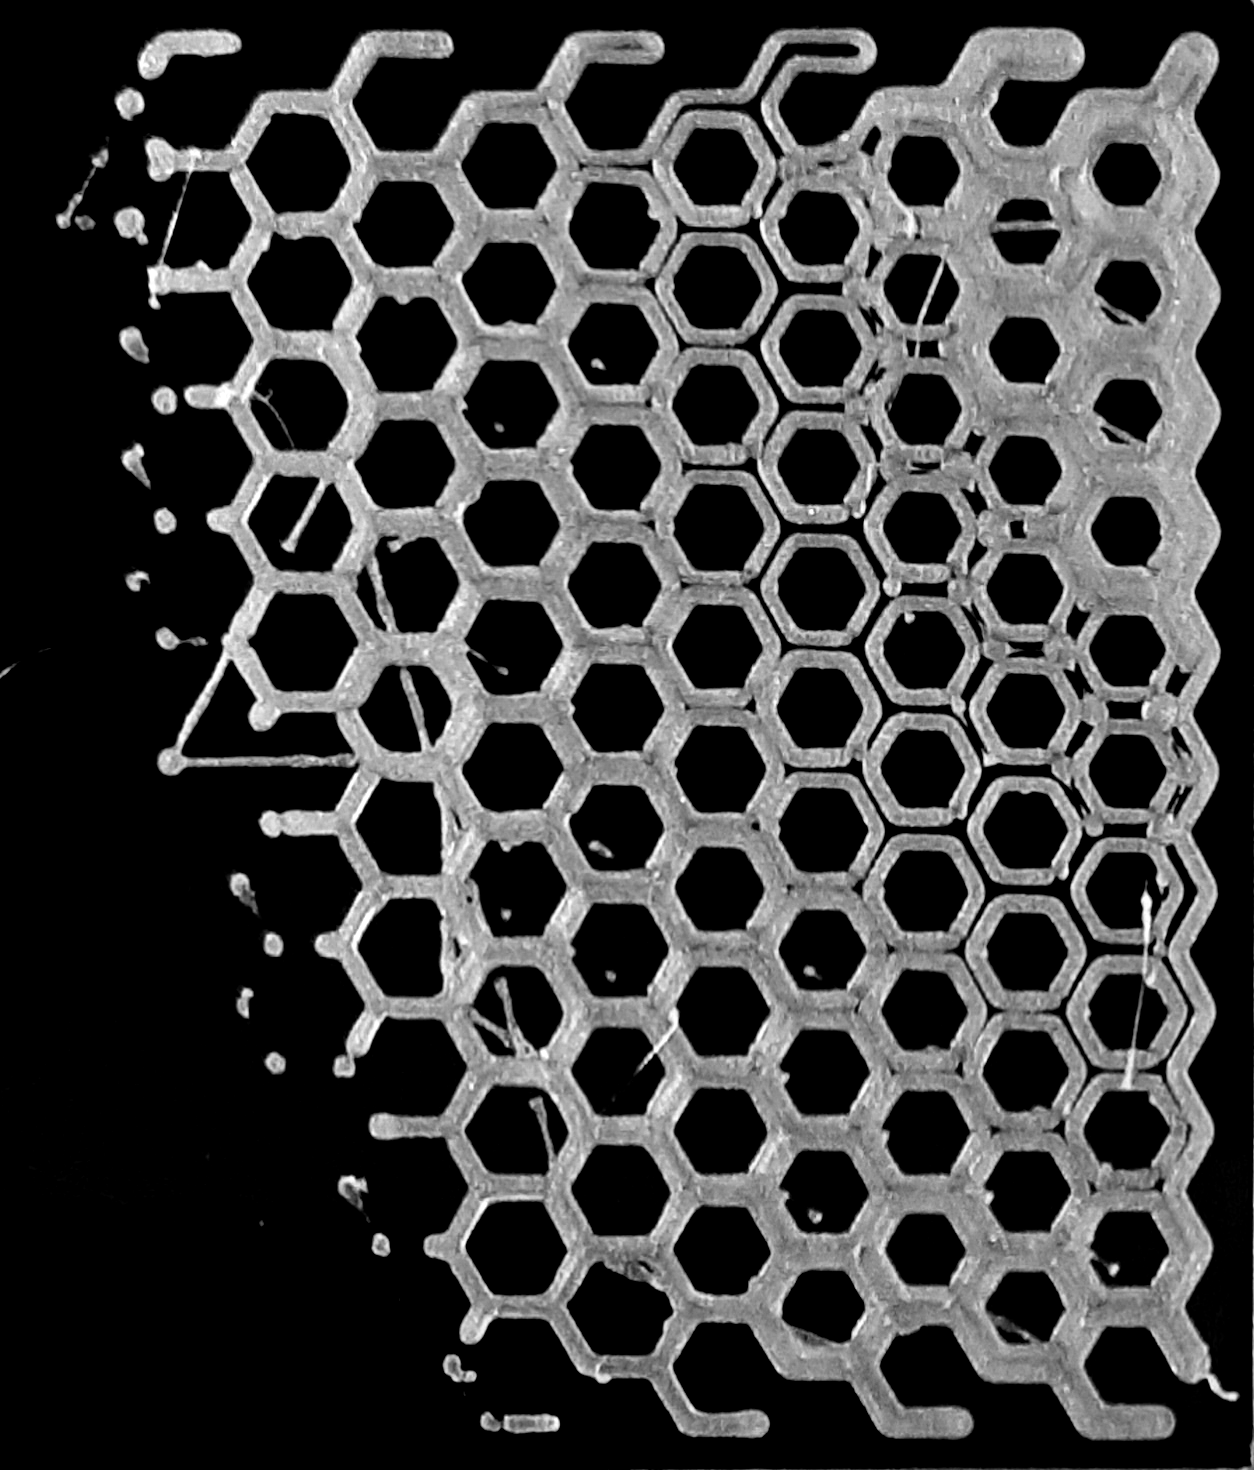
\includegraphics[height=\figheight]{sources/applications/P3_print_hex_naive_edited.png}

\includegraphics[width=\figwidth]{sources/applications/P3_print_UM_naive_edited.png}
\caption{Naive}\label{print_naive}
\end{subfigure}
\begin{subfigure}{\figwidth}\centering
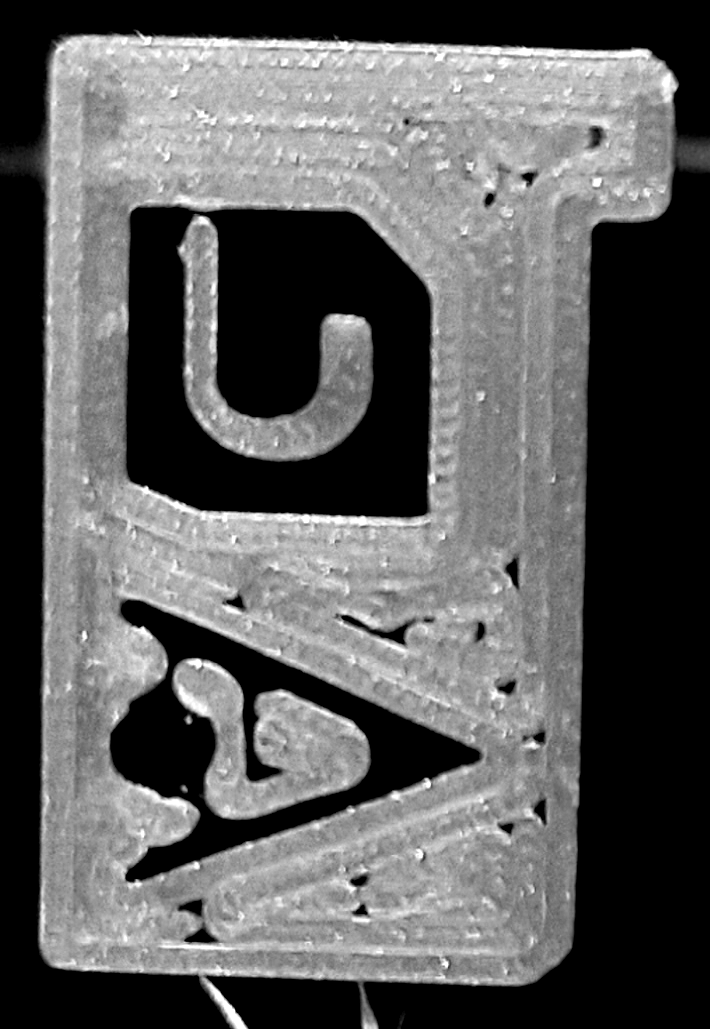
\includegraphics[height=\figheightTwo]{sources/applications/gMAT_center.png}
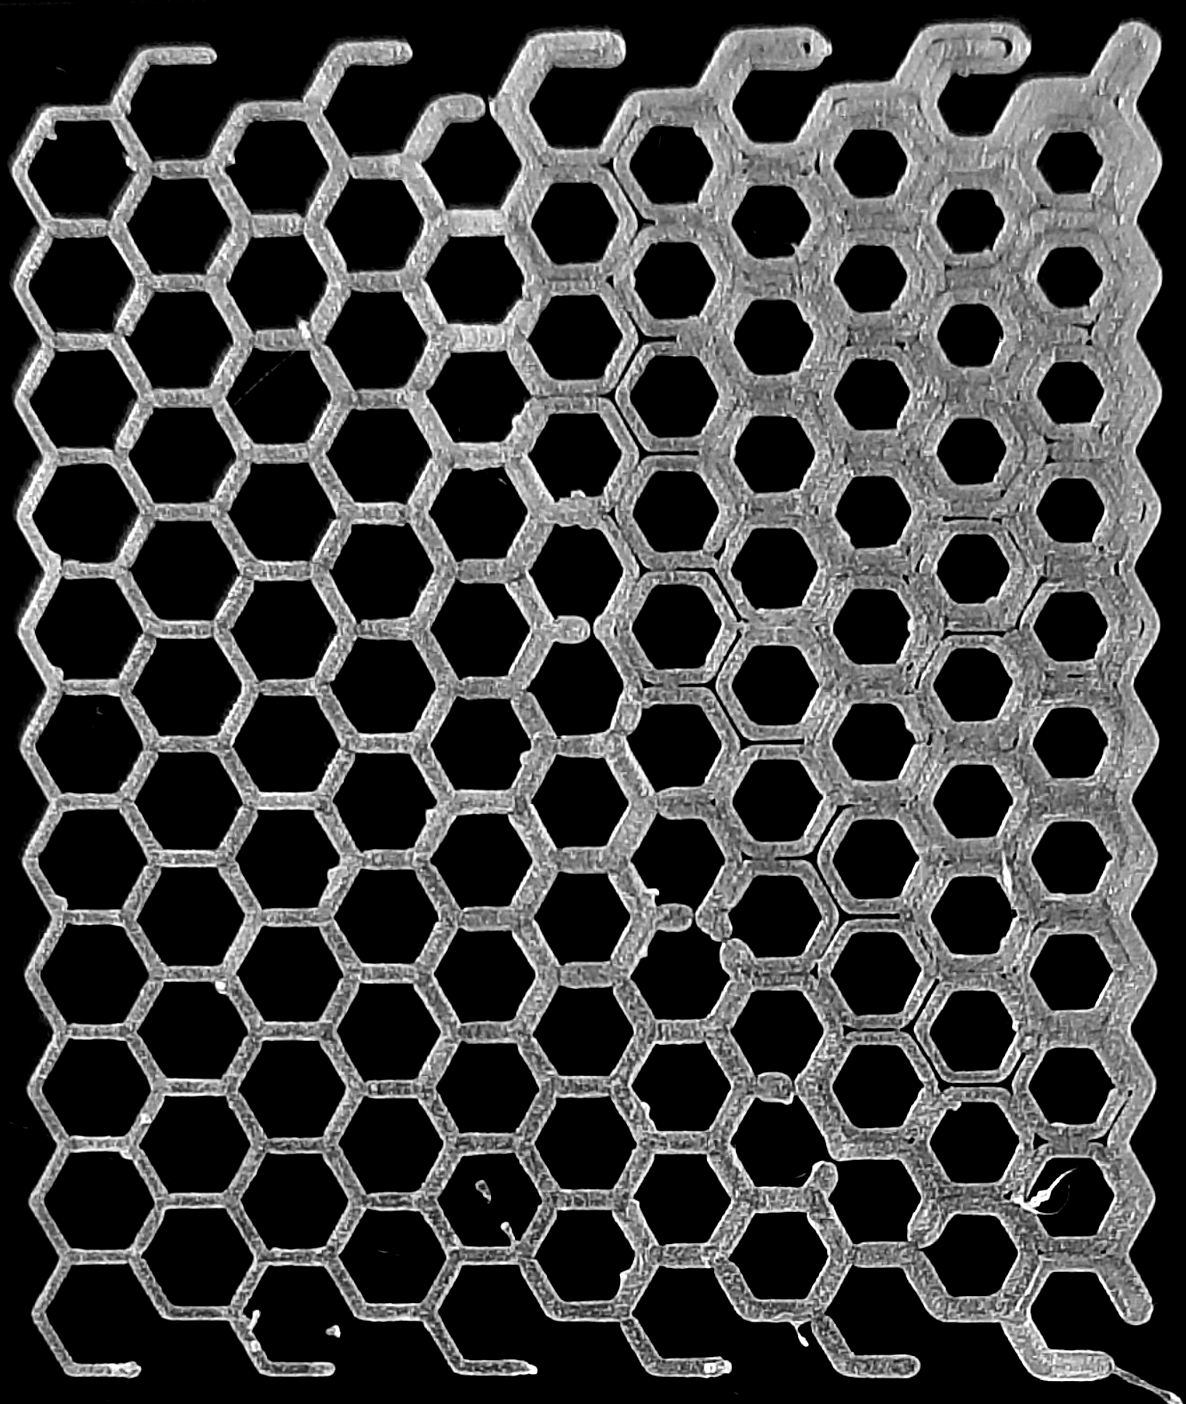
\includegraphics[height=\figheight]{sources/applications/P3_print_hex_center_edited.png}

\includegraphics[width=\figwidth]{sources/applications/P3_print_UM_center_edited.png}
\caption{Center deviation}\label{print_center}
\end{subfigure}
\begin{subfigure}{\figwidth}\centering
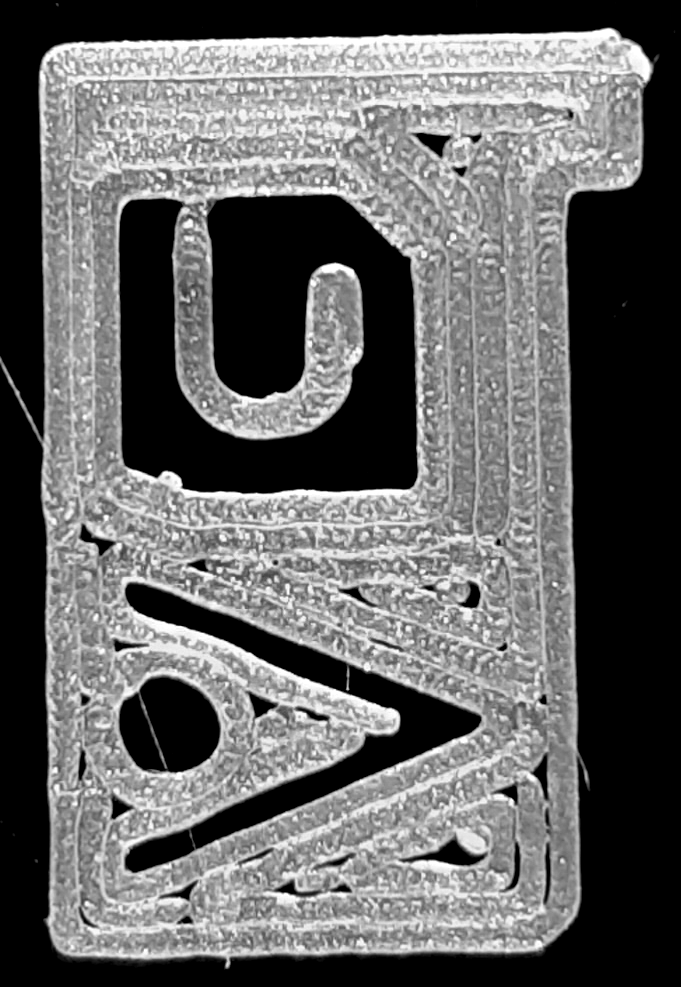
\includegraphics[height=\figheightTwo]{sources/applications/gMAT_inward.png}
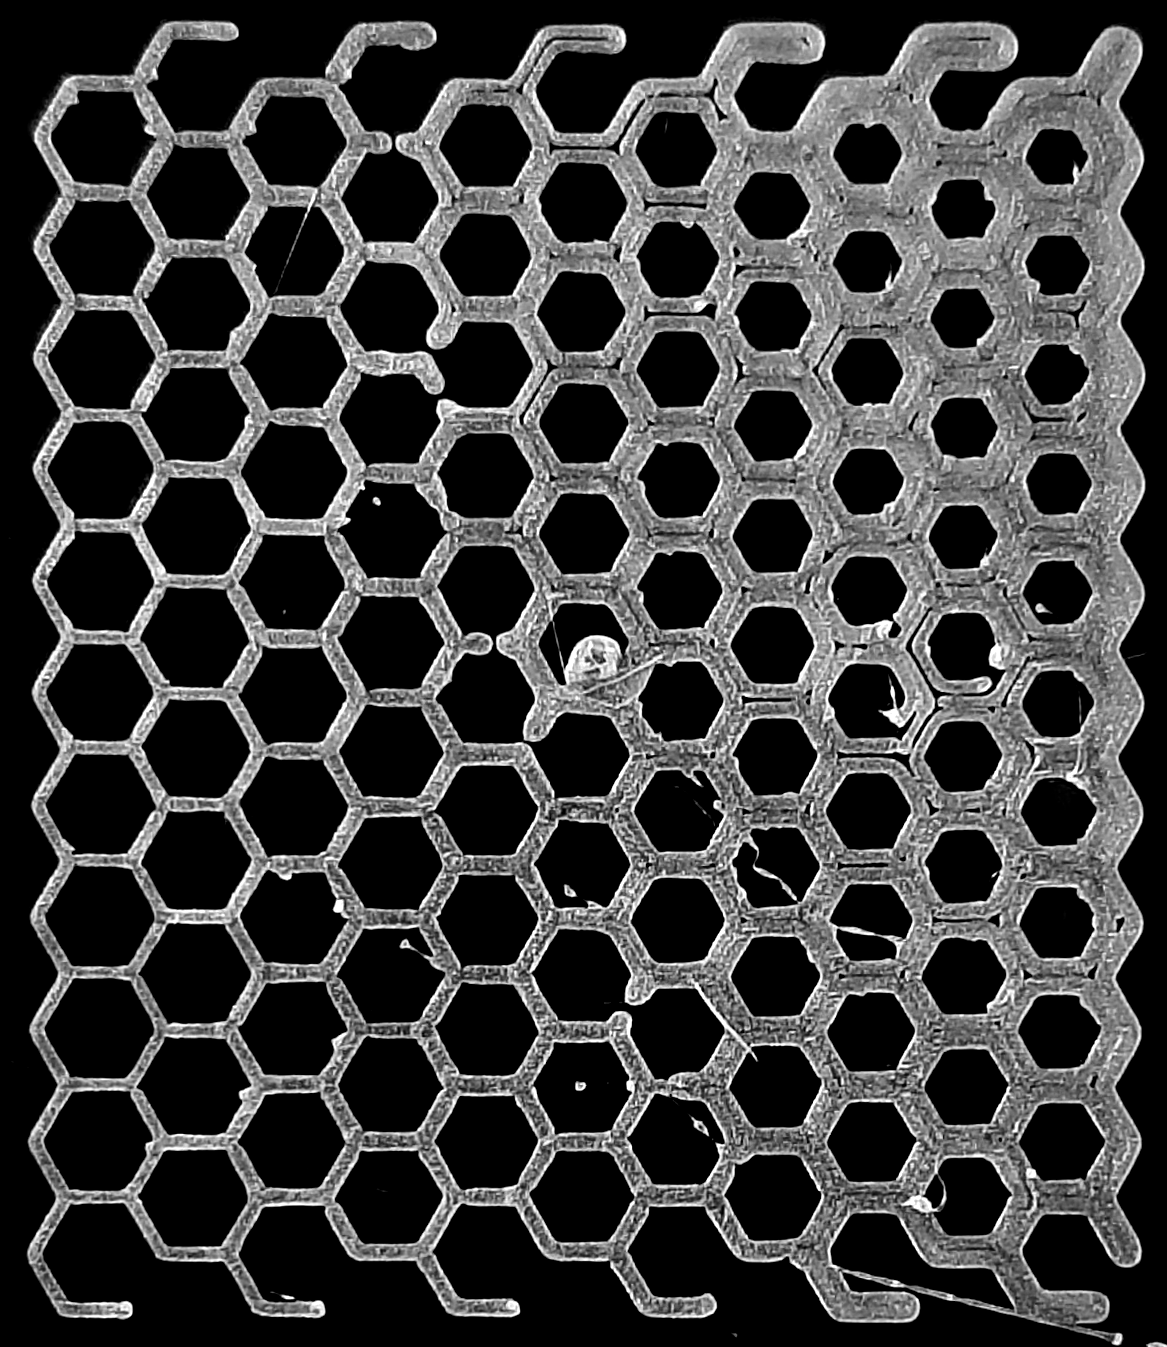
\includegraphics[height=\figheight]{sources/applications/P3_print_hex_inward_edited.png}

\includegraphics[width=\figwidth]{sources/applications/P3_print_UM_inward_edited.png}
\caption{Inward distributed}\label{print_inward}
\end{subfigure}
\caption{
Test shapes printed using the naive strategy, center deivation strategy and the inward distributed strategy.
The naive method produces distinct underfill areas.
The center deviation strategy shows some defects due to inaccurate control of extremal deposition widths.
The inward distributed strategy produces the least defects.
}
\label{prints}
\end{figure}


\iffalse
\todo{Maybe test the following qualities:}
\begin{itemize}
\item visual consistency of flat top skin surface
\item graphs of tensile tests on thin walled object
\end{itemize}
\fi










%We therefore visualize include a semi-circle with a diameter equal to the starting width in the one end, and exclude it at the other end, because it will be included in the next extrusion segment.


